\documentclass[twoside,twocolumn]{article}


% \usepackage[sc]{mathpazo} % Use the Palatino font
\usepackage[T1]{fontenc} % Use 8-bit encoding that has 256 glyphs
\linespread{1.05} % Line spacing - Palatino needs more space between lines
\usepackage{microtype} % Slightly tweak font spacing for aesthetics


\usepackage[english]{babel} % Language hyphenation and typographical rules

\usepackage[hmarginratio=1:1,top=32mm,columnsep=20pt, margin=2cm]{geometry} % Document margins
\usepackage[small,labelfont=bf,up,textfont=it,up]{caption} % Custom captions under/above floats in tables or figures
\usepackage{booktabs} % Horizontal rules in tables

\usepackage{enumitem} % Customized lists
\setlist[itemize]{noitemsep} % Make itemize lists more compact

\usepackage{abstract} % Allows abstract customization
\renewcommand{\abstractnamefont}{\normalfont\bfseries} % Set the "Abstract" text to bold
% \renewcommand{\abstracttextfont}{\normalfont\small\itshape} % Set the abstract itself to small italic text

\usepackage{titlesec} % Allows customization of titles
\titleformat{\section}[block]{\large\scshape\centering}{\thesection.}{1em}{} % Change the look of the section titles
\titleformat{\subsection}[block]{\large}{\thesubsection.}{1em}{} % Change the look of the section titles

\usepackage{titling} % Customizing the title section

\usepackage{cite}
% \addbibresource{report.bib}
\usepackage{siunitx}
\sisetup{
    separate-uncertainty = true,
    % multi-part-units = single
    }
\DeclareSIUnit \parsec {pc}

\usepackage{bm}
\usepackage{braket}
    
\usepackage{graphicx}
\usepackage{array}
\newcolumntype{P}[1]{>{\raggedright\arraybackslash}p{#1}}
\usepackage{url}
\usepackage{amsmath}

\usepackage{listings}

%----------------------------------------------------------------------------------------
%	TITLE SECTION
%----------------------------------------------------------------------------------------

\setlength{\droptitle}{-4\baselineskip} % Move the title up

\pretitle{\begin{center}\Huge\bfseries} % Article title formatting
\posttitle{\end{center}} % Article title closing formatting
\title{Tidal Tails and Interacting Galaxies} % Article title
\author{%
    \normalsize University of Cambridge \\ % Your institution
    }
\date{
    \today \\
} % Leave empty to omit a date

\renewcommand{\maketitlehookd}{%

\begin{abstract}
    A tidal tail is a long, thin region of stars and interstellar dust extending from a galaxy, and is a result of gravitational forces between interacting galaxies. A simple N-body simulation of two interacting galaxies was performed where specifically, a star-less perturbing galaxy with initial conditions of a parabolic orbit was introduced to a central galaxy with circularly orbiting stars. The simulation showed that the tidal tail was created from the outer orbiting stars of the central galaxy. Quantitative results, such as the fraction of stars disturbed from their initial orbits, were obtained for different characteristics and initial conditions of the perturbing galaxy. Varying the distance of closest approach of the two galaxies showed that a larger fraction of stars were disturbed when the distance of closest approach is smaller. Changing the mass of the perturbing galaxy demonstrated that the heavier the perturbing galaxy, the more stars that were stripped away from the central galaxy. [Word count: 2408]

    
\end{abstract}
}


\begin{document}

\maketitle

\section{Introduction}
    Tidal tails are long, thin, often curved regions made up of stars and interstellar debris extending from a galaxy, and is a result of the strong tidal gravitational forces of interacting galaxies. Tidal tails are often used to study and characterise the evolution of galactic phenomena, including galaxy mergers and tidal dwarf galaxies \cite{alavi}. A well-known example of tidal tails are the Antennae Galaxies, which are a pair of galaxies that are currently undergoing galactic collision. The system's pair of prominent tidal tails can be seen in Figure \ref{figure:antennae}, and is what gives its characteristic insect-like outline. Another example can be observed in the Tadpole Galaxy, where its long tidal tail of approximately \SI{86}{\kilo\parsec} has been attributed to a merger with a smaller galaxy in the past \cite{tadpole}. This can also be seen in Figure \ref{figure:antennae}.   
    
    \begin{figure}
        \centering
        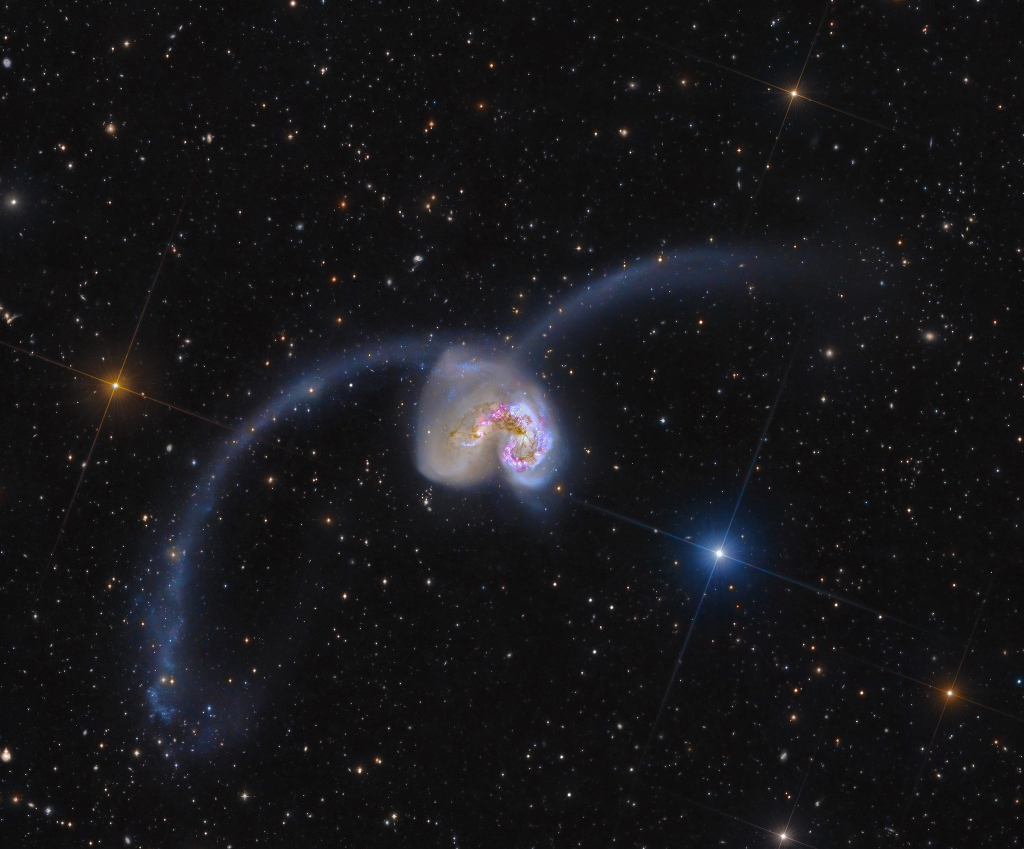
\includegraphics[width=0.9\linewidth]{images/antennae.png}

        \vspace{0.2cm}
        
        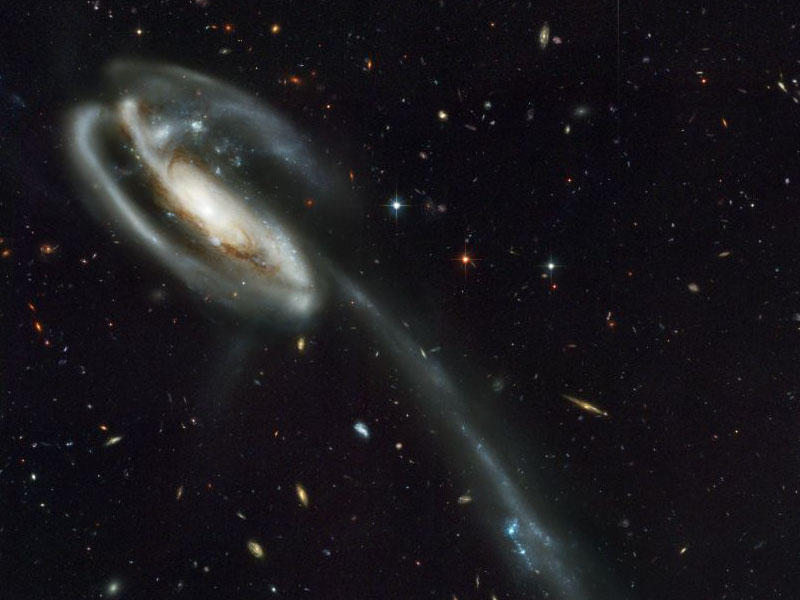
\includegraphics[width=0.9\linewidth]{images/tadpole_tail.png}
        \caption{Top image: The Antennae Galaxies. A pair of prominent tidal tails can be seen extending from both sides of the system. Bottom image: Tadpole Galaxy. Its characteristic long tidal tail can be seen extending from the core of the galaxy.}
        \label{figure:antennae}
        
    \end{figure}

    In one of the first simulations of the interaction between multiple galaxies by Toomre and Toomre in 1972 \cite{toomre}, they found that tidal tails were primarily formed through prograde encounters between the 'central' and perturbing galaxy, where both the stars in the 'central' galaxy and the perturbing galaxy are orbiting in the same direction. Toomre and Toomre used the restricted three-body equations of motion, alongside the fourth-order Runge-Kutta method in order to simulate the interaction. A few years later, Keenan and Innanen investigated the same effects using numerical methods, and came to the same conclusion \cite{keenan}. Their studies were able to reconstruct the appearance and outer outlines of a number of galactic systems, including Arp 295, M51 + NGC 5195, NGC 4676 and the Antennae Galaxies.

    Just like in the experiments mentioned above, the aim of this investigation is to run a simple N-body simulation of two interacting galaxies, which shall be called the \emph{central} and \emph{perturbing} galaxies. The central galaxy will contain test particles, which represent the stars, orbiting around a central heavy mass at multiple radii. Given that the masses of stars are negligible compared to the central mass of a galaxy, the test particles' masses will be assumed to be 0. A perturbing galaxy will be introduced with the initial conditions of a parabolic orbit, and the effects of the perturbing galaxy will be observed.


\section{Analysis}    

    The main concern of this investigation into interacting galaxies is the N-body simulation method that will be used. As stated by Toomre and Toomre in their paper, there are two simple methods that can be used for such simulations: the timestep method, or integrating the restricted three-body equations of motion with the fourth-order Runge-Kutta method. There are also more modern and sophisticated techniques such as tree methods (Barnes-Hut) and particle mesh methods that reduces the runtime of the program, but these are ignored due to this investigation being rather small scale, thus not requiring the need for such efficiency. The timestep and restricted three-body methods for a single test particle are outlined below:
    \vspace{0.2cm}

    \textbf{Timestep method}
    \begin{enumerate}
        \item Provide the initial position and velocity of the test particle.
        \item Calculate the forces acting on the test particle, resolving them in each axis direction. Working in 2 dimensions, the gravitational acceleration acting in each axis direction caused by a massive object is
        \begin{equation}
            \ddot{x} = \frac{GM(x - X)}{r^3}, \ \ \ddot{y} = \frac{GM(y - Y)}{r^3}
            \label{eqn:acceleration}
        \end{equation}
        where $G$ is the gravitational constant, $M$ is the mass of the massive object, $(x, y)$ is the position of the test particle, $(X, Y)$ is the position of the massive object and $r = \sqrt{(x - X)^2 + (y - Y)^2}$. 
        \item Let $\delta t$ be a small timestep. Thus the velocity, as a result of the acceleration caused by the gravitational force, is
        \begin{equation}
            \dot{x} = \dot{x}_0 + \ddot{x} \delta t, \ \ \dot{y} = \dot{y}_o + \ddot{y} \delta t
        \end{equation}
        and the position is
        \begin{equation}
            x = x_0 + \dot{x} \delta t, \ \ y = y_0 + \dot{y} \delta t
        \end{equation}
        where $(x_0, y_0)$ and $(\dot{x}_0, \dot{y}_0)$ are the initial position and velocity of the test particle.
        \item Repeat these steps until the end time is reached.
    \end{enumerate}
    \vspace{0.2cm}

    \textbf{Restricted three-body method}
    \begin{enumerate}
        \item The acceleration of the test particle is given by the same equation (Equation \ref{eqn:acceleration}) as in the timestep method. For the three-body system, the equation of motion is given as \cite{three_body}
        \begin{equation}
            \begin{split}
                &\ddot{x} = - \frac{GM_1(x - X_1)}{r_1^3} - \frac{GM_2(x - X_2)}{r_2^3} \\
                &\ddot{y} = - \frac{GM_1(y - Y_1)}{r_1^3} - \frac{GM_2(y - Y_2)}{r_2^3},
            \end{split}
        \end{equation}
        where $M_{1,2}$ are the masses of the massive objects, $(X_{1, 2}, Y_{1, 2})$ are the positions of the massive objects and $r_{1, 2}$ are the distances between the test particle and the massive objects. 
        \item Two first order ODEs in each axis direction are obtained from the equation of motion. The fourth-order Runge-Kutta method is then used here to integrate the first order ODEs for each test particle.
        \item The motion of the test particle is then known based off the motion of the two massive interacting bodies.
    \end{enumerate}
    
    \begin{figure}
        \centering
        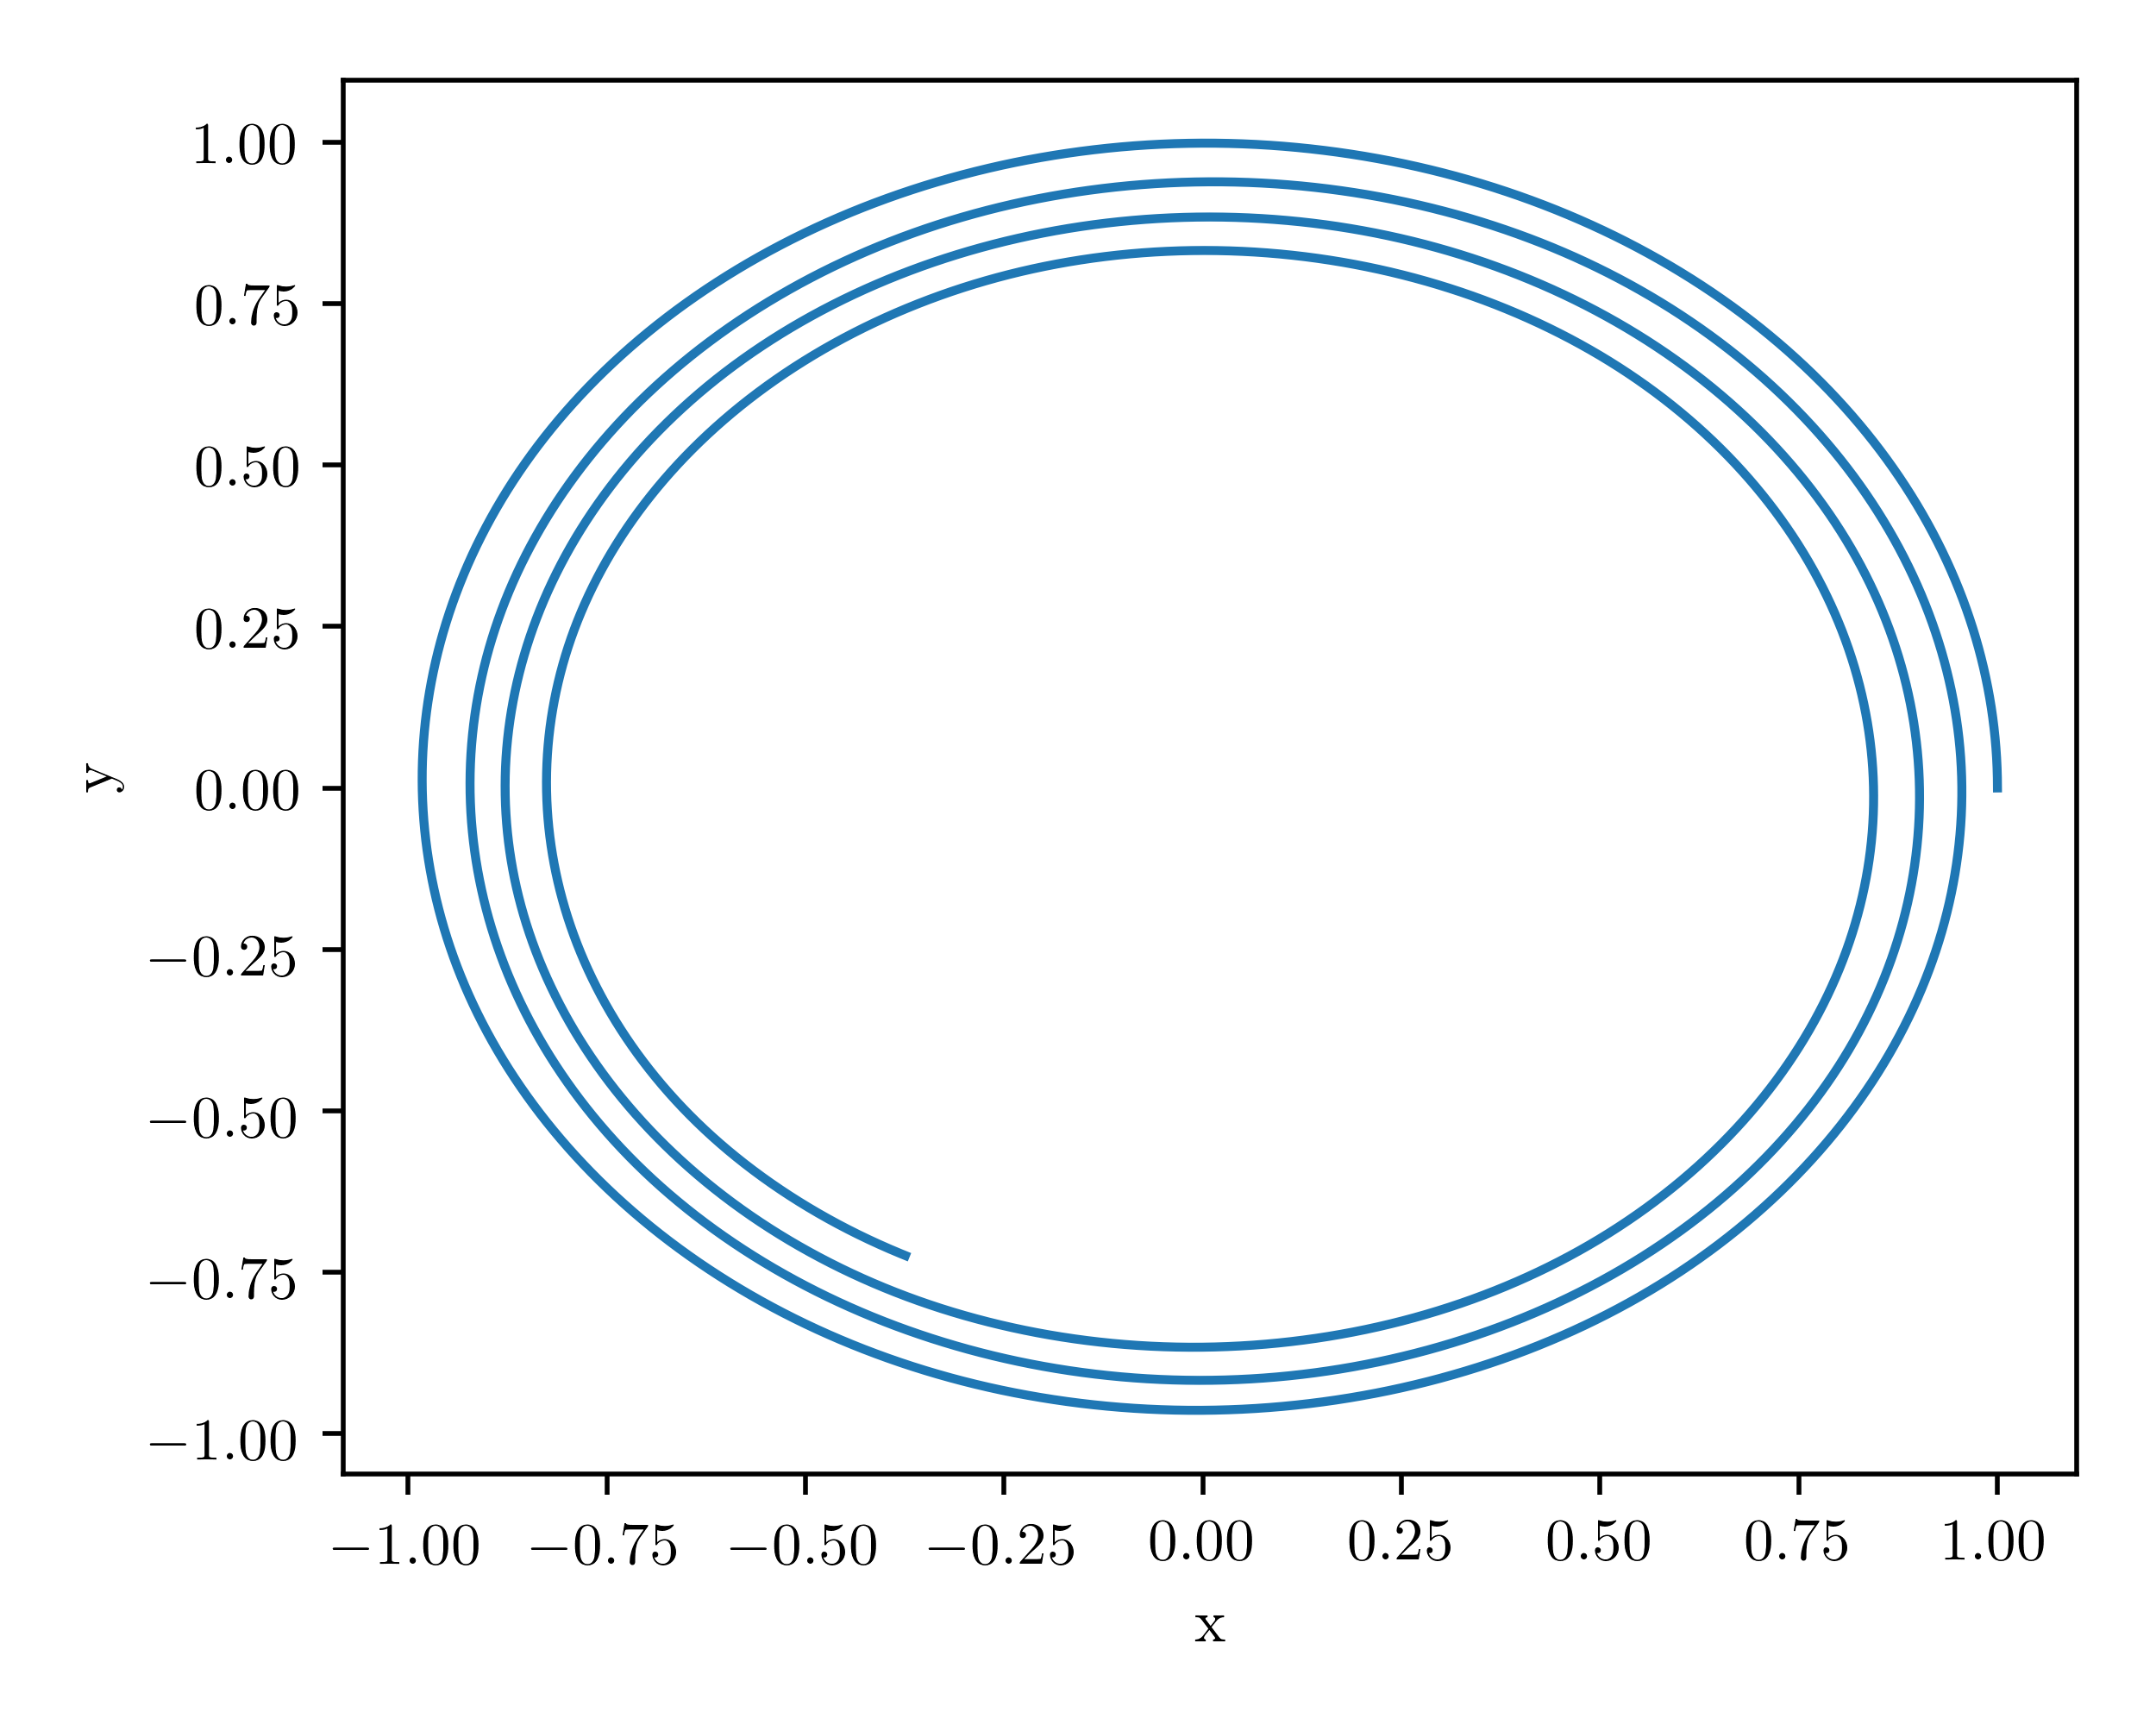
\includegraphics[width=\linewidth]{images/RK45.png}
        \caption{With the central mass positioned at $(0, 0)$ and the test particle having an initial velocity $v = \sqrt{GM/r}$, the path of the test particle spirals inward when the fourth-order Runge-Kutta method is used to integrate its equation of motion.}
        \label{figure:RK45}
        
    \end{figure}

    In order to determine the preferred technique, these two methods were tested on a simple two-body system consisting of a large mass and a circularly orbiting test particle. This small experiment showed that the Runge-Kutta method losed its accuracy quickly for orbiting systems such as this one, where the path of the test particle was found to spiral inward, as shown in Figure \ref{figure:RK45}. The timestep method, despite being more inefficient, proved to be more accurate for such a system. Thus, the timestep method was the method of choice for this investigation.

    Another key computational aspect in this investigation was the use and storage of the calculated particle trajectories. Knowing that the simulation will contain many test particles, potentially $>1000$ particles, it was important to keep in mind that a good system to store and read the calculated data was required. Such a system would most likely need to be able to create and read multiple large \texttt{.csv} files for the experiments that will be performed.    
    

\section{Implementation}

    This N-body simulation contained 1200 test particles of zero mass orbiting circularly around the central galaxy, where 120, 180, 240, 300 and 360 particles orbited at a radius of 2, 3, 4, 5 and 6 units. The perturbing galaxy contained no test particles, and it had the initial conditions of a parabolic orbit about the central galaxy. The test particles experienced the gravitational forces of both massive galaxies, whilst both galaxies experienced the gravitational force from one another. Note that the gravitational constant $G = 1$ in this simulation, and units were generally disregarded here.

    A few experiments were performed, and they are given below:
    \begin{itemize}
        \item comparing prograde and retrograde encounters,
        \item varying the mass of the disrupting galaxies,
        \item and varying the distance of closest approach.
    \end{itemize}
    A single quantitative metric was used here, which is the fraction of test particles disturbed from their initial orbits, where the definition of disturbed is when the test particle deviates from its original radius by $>0.5$.

    \subsection{Physics}
        \label{section:physics}

        For test particles to orbit around the central galaxy in a stable circular fashion, suitable initial velocities were required. Equating the centripetal force and the gravitational force, a test particle required its velocity $\bm{v}$ to have a magnitude $\lvert\bm{v}\lvert = \sqrt{GM/r}$, travelling perpendicular to the radius. The velocities in the $x$ and $y$ direction could then be written as $v_x = - \lvert\bm{v}\lvert \sin{\theta}$ and $v_y = \lvert\bm{v}\lvert \cos{\theta}$, where $\theta$ is the angle between the positive x-axis and position vector of the test particle relative to the central galaxy. Note that the test particles were orbiting in an anti-clockwise manner here.


        A parabolic orbit has the characteristic of the system having zero net energy, where the kinetic energy is balanced with the gravitational potential energy. This is given as
        \begin{equation}
            E = 0 = \frac{mv^2}{2} - \frac{GMm}{r}, \ \lvert\bm{v}\lvert = \sqrt{\frac{2GM}{r}}
        \end{equation}
        where $M$ is the mass of the central mass, $m$ is the mass of the orbiting mass, $\bm{v}$ is the velocity of the orbiting mass and $r$ is the distance between the central and orbiting masses. A parabolic orbit also has a trajectory given by \cite{lecture}
        \begin{equation}
            y^2 = 4r_{min}^2 - 4r_{min}x,
        \end{equation}
        where $r_{min}$ is the minimum distance of approach of the orbiting mass. The initial velocities of the perturbing mass in the $x$ and $y$ direction can then be determined using the fact that $v^2 = v_x^2 + v_y^2$ and the derivative of the trajectory $y' = dy/dx = v_x/v_y$. Combining these equations give
        \begin{equation}
            v_y = \frac{y'\lvert\bm{v}\lvert}{\sqrt{1 + y'^2}}, \ v_x = \frac{v_y}{y'}.
        \end{equation}
        It was important to keep track of the signs here since the perturbing galaxy could be introduced either prograde or retrograde with respect to the orbiting test particles.
    
    \subsection{Code}
        A \texttt{Body} class was created to represent both the massive galaxies and test particles. This class contained two key functions, \texttt{set\_gforce} and \texttt{update\_speed\_position}, which obtained the resultant forces acting on the body and updated the body's speed and position respectively.

        in the first script, The initial positions of the test particles were initialised at random angles $\theta$ for each radii. The initial velocities of the test particles and perturbing galaxy were obtained using the equations from \S \ref{section:physics}. A small timestep  of \texttt{dt = 0.1} was used to iterate through from \texttt{t = 0} to \texttt{t = 1000}, where the two instance methods of the \texttt{Body} class were called each time for each test particle and mass instance. At each iteration, the positions of the test particles and masses were also written into a new line in a \texttt{.csv} file.
        
        The second script was used to read the \texttt{.csv} files, which in turn was used to visualise and quantify the outcome of the simulation. Both scripts can be found in the appendix. 


\begin{figure*}
    \centering
    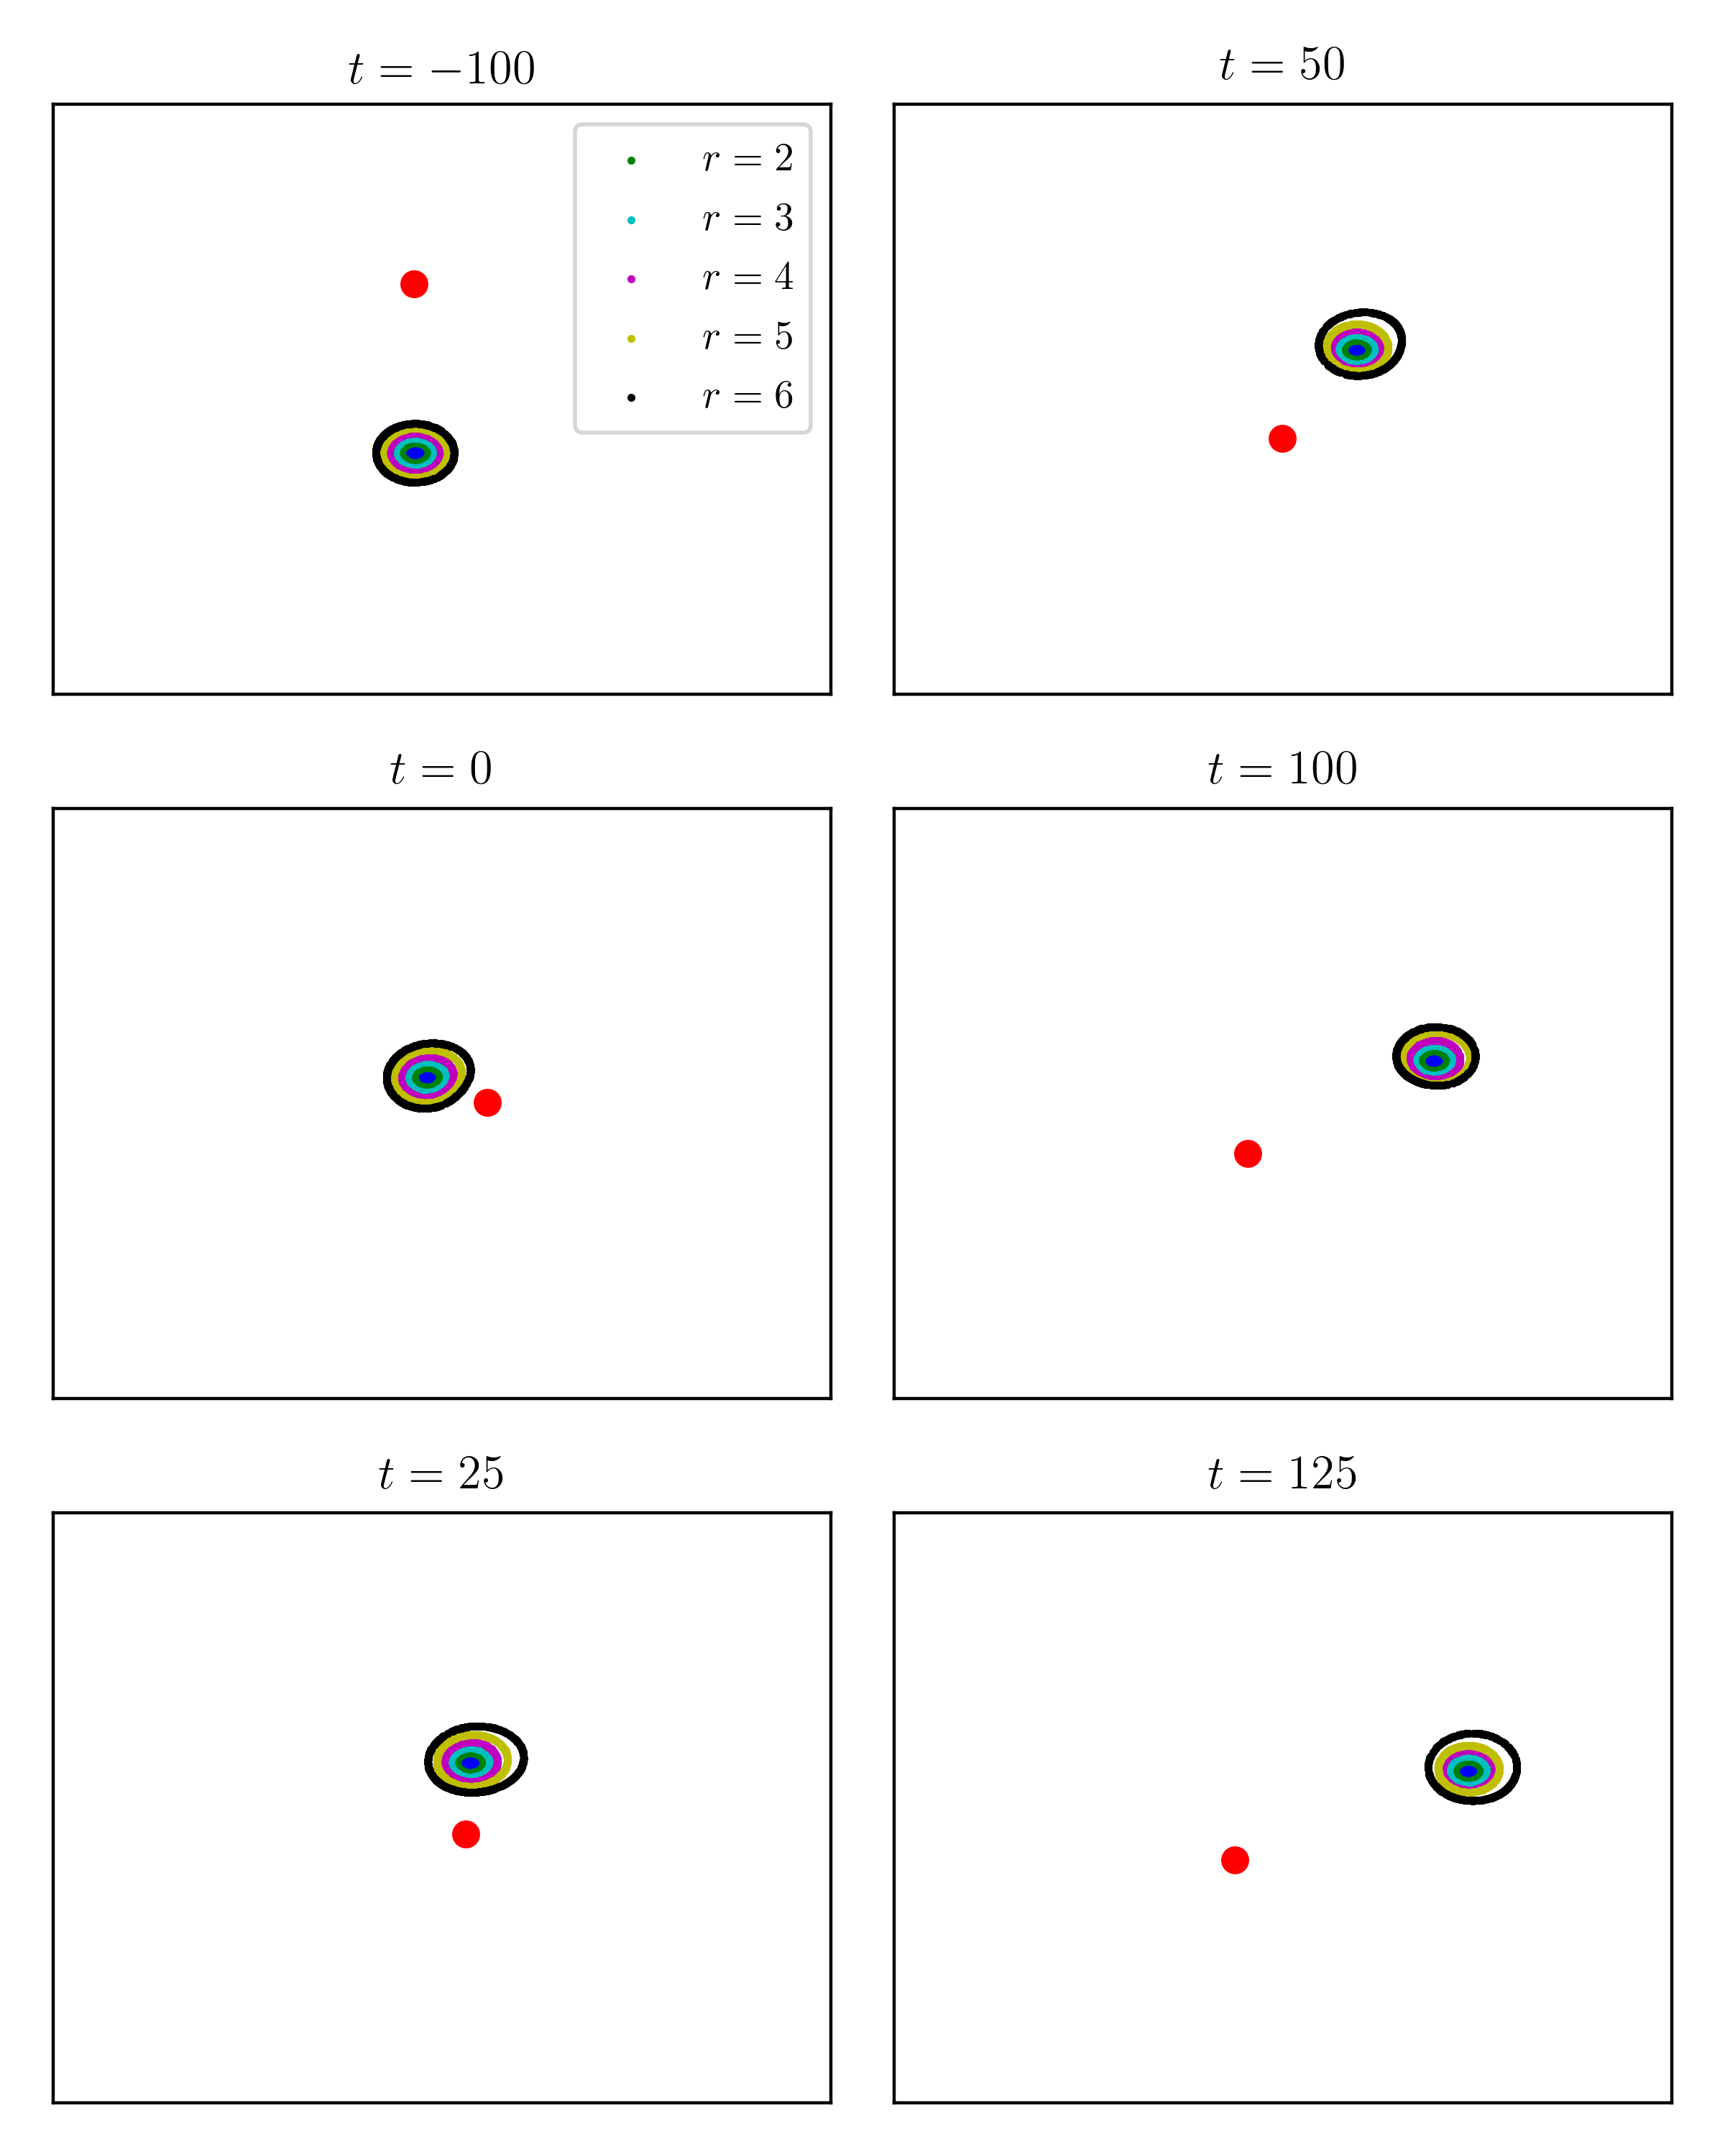
\includegraphics[width=\linewidth]{images/clockwise_positions.png}
    \caption{A time evolution of the retrograde encounter between the two galaxies. Notice that none of the stars are thrown out of orbit, however the outer orbiting stars seem to have its orbit destabilised.}
    \label{figure:retrograde}
\end{figure*}

\begin{figure*}
    \centering
    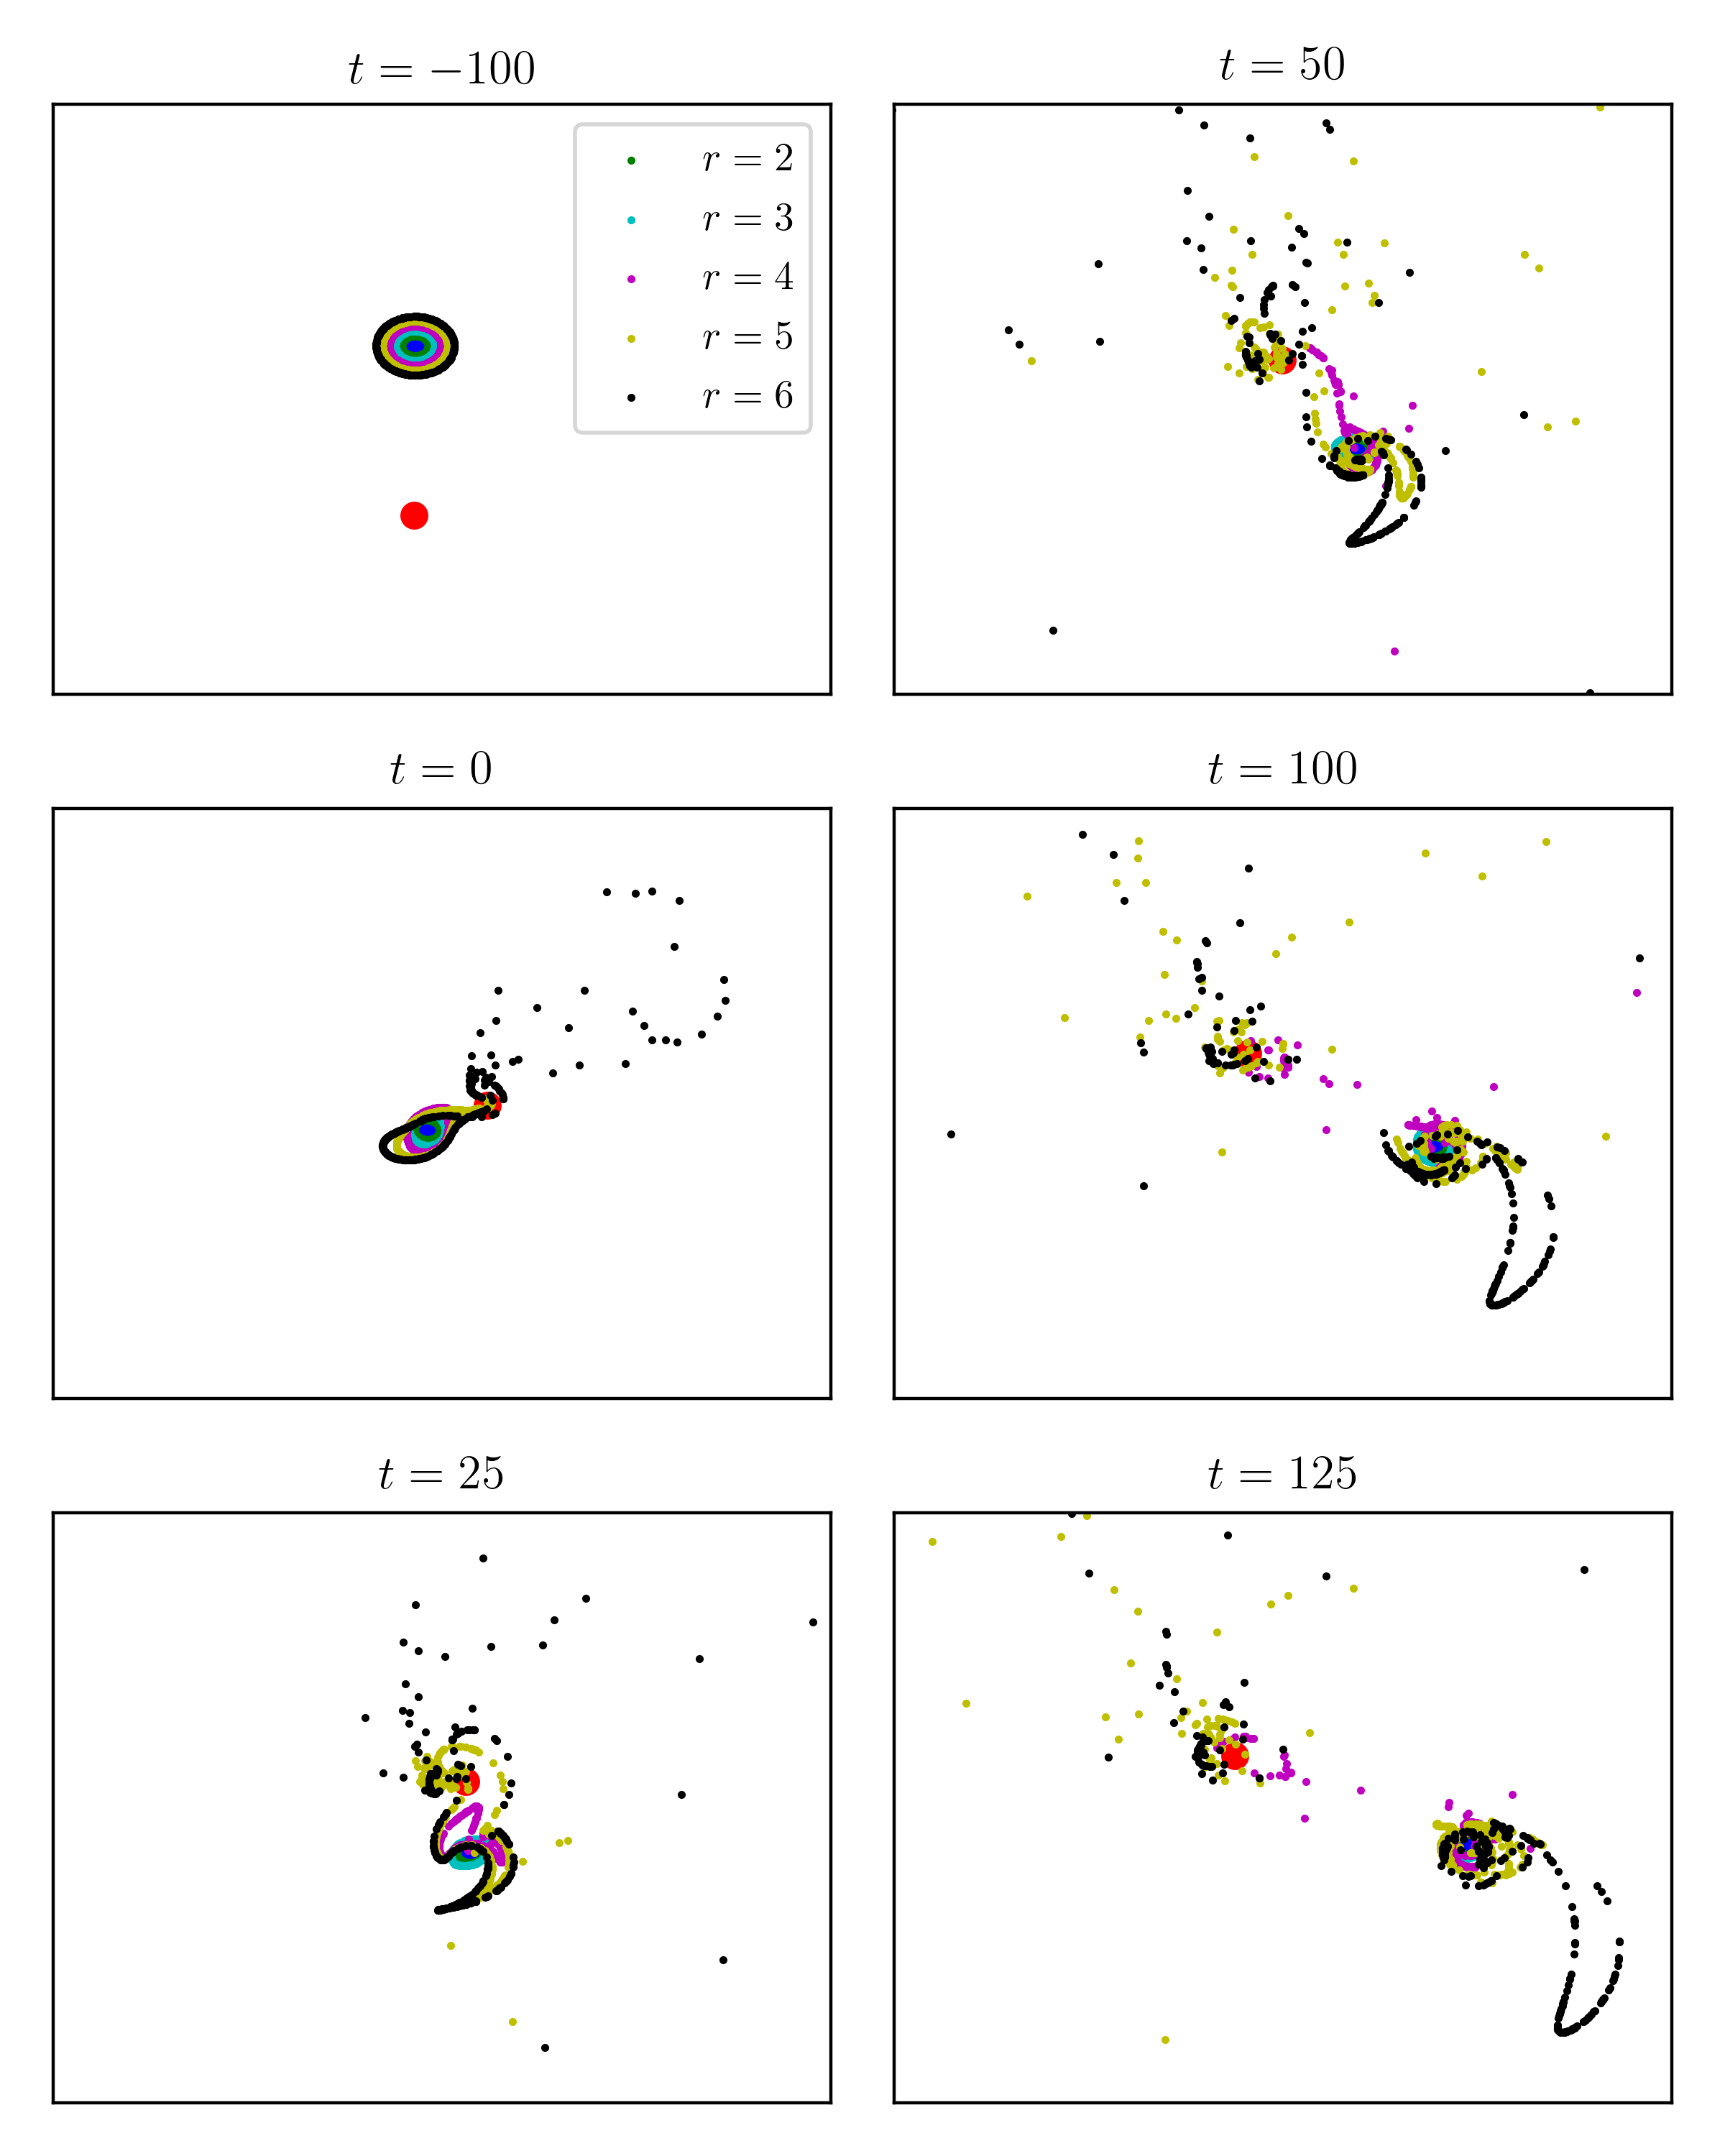
\includegraphics[width=\linewidth]{images/anticlockwise_positions.png}
    \caption{A time evolution of the prograde encounter between the two galaxies. The final two snapshots of the encounter show the development of a tidal tail made up of stars from the outer orbits of the central galaxy.}
    \label{figure:prograde}
\end{figure*}    


    \subsection{Performance}

        Given the large number of test particles, the simulation was expected to take some time to run, especially given the limitations of the hardware of a laptop. Particular attention was given to using Python's list comprehension rather than using loops in order to improve the runtime of the program. One run of the simulation took on average around \SI{100}{\second}.

        When it came to reading the large \texttt{.csv} files, the main bottleneck was loading the contents of the file into memory. Two known built-in methods that does this are \texttt{numpy}'s \texttt{loadtxt} and \texttt{pandas}'s \texttt{read\_csv} methods. It was found that \texttt{pandas.read\_csv} method was significantly faster than \texttt{numpy.loadtxt}, where \texttt{pandas.read\_csv} took around \SI{9}{\second} whereas \texttt{numpy.loadtxt} took around \SI{22}{\second}. Thus, the \texttt{pandas} method was used here.

        
\section{Results and Discussion}

    A small program using \texttt{matplotlib} was used to animate the evolution of the system with scatter plots. This program allowed the simulation to be verified visually to be working as expected. The following results the sections below were also used to verify that the simulation was working as expected, since this simulation produced similar results to those performed by Toomre and Toomre.
    

\subsection{Prograde and Retrograde Encounters}

        Figure \ref{figure:retrograde} and \ref{figure:prograde} show the retrograde and prograde encounters of the two galaxies respectively. Multiple runs of the same simulation were performed, and very similar results were obtained from them. The figures show a clear agreement between the results of this simulation and those performed by Toomre and Toomre, where the prograde encounter is shown to have a significantly more disruptive effect than the retrograde encounter. 
        
        In the retrograde encounter, there is a noticeable destabilisation of the outermost circular orbit in the last four snapshots. However, the outermost stars remain in orbit, albeit not circular, around the central galaxy. This mild effect can possibly be attributed to weak tidal effects from the perturbing galaxy, where the velocities of the test particles nearest to the perturbing galaxy have similar directions to the velocity of the perturbing galaxy.  In the prograde encounter, strong tidal effects, arising from the large difference in the direction of the velocities of the test particles and perturbing galaxy, tear apart the outer stars with an orbiting radius of 4, 5 and 6 units. The formation of the tidal tail, which is made up of the outermost stars, seen in the last four snapshots is the most noticeable effect of such strong tidal forces. A large proportion of the outer stars were also 'absorbed' by the perturbing galaxy, where these stars form new orbits around the perturbing galaxy.

    \subsection{Varying Initial Conditions of Perturbing Galaxy}

        \begin{figure}
            \centering
            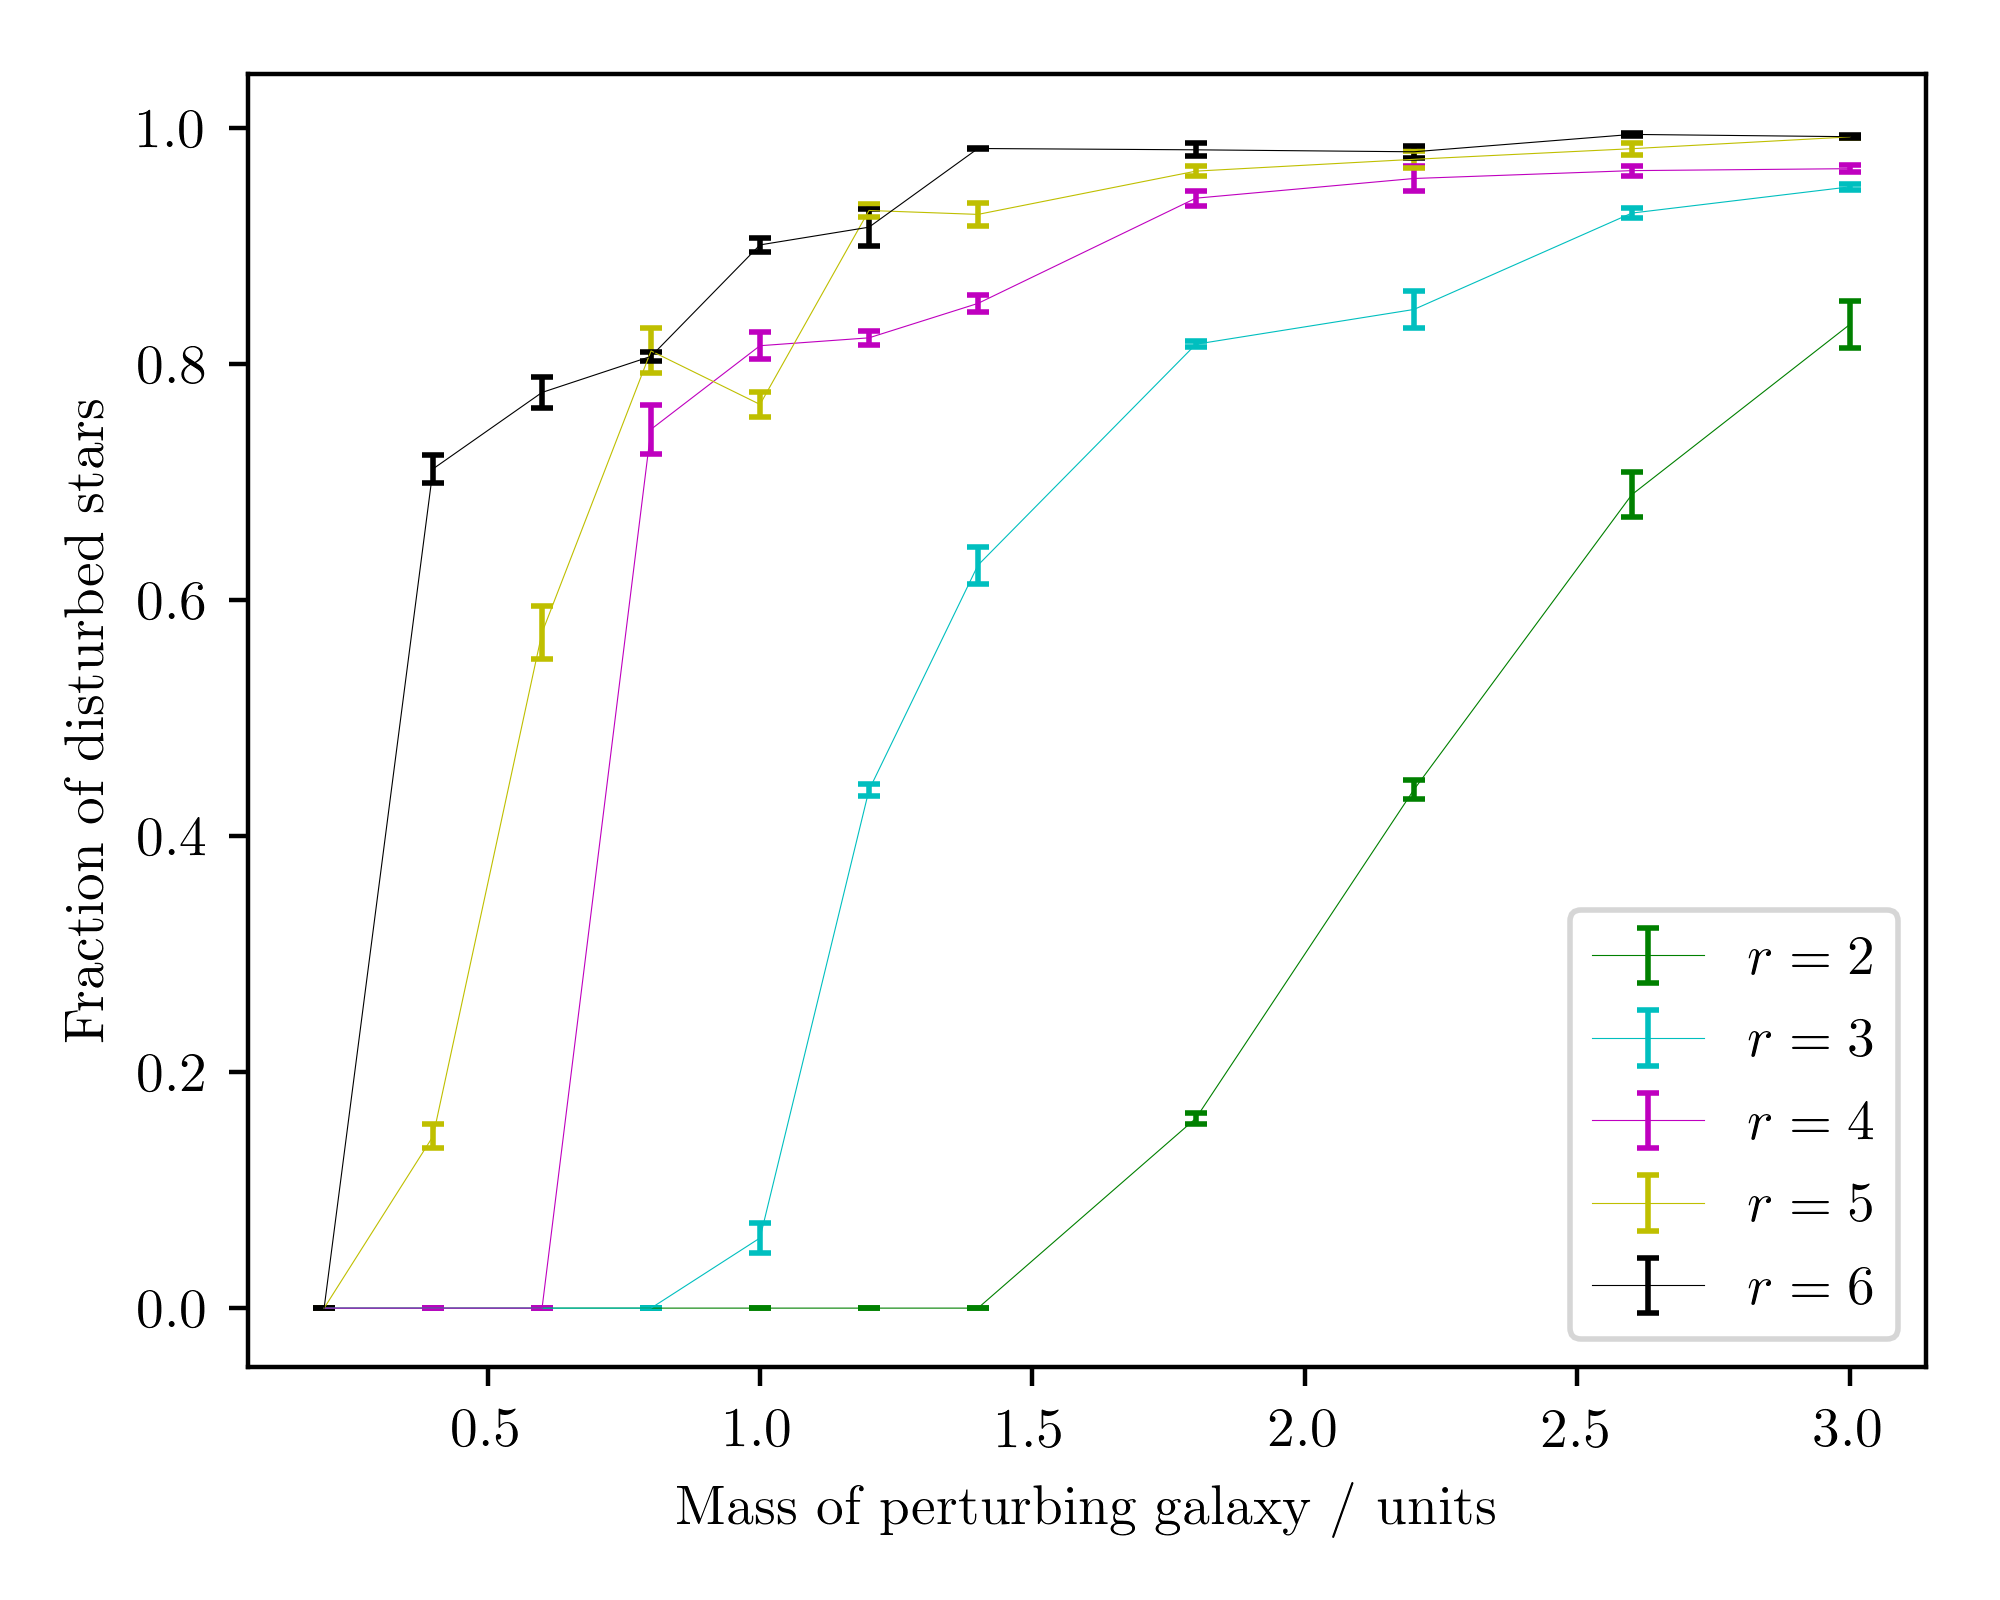
\includegraphics[width=\linewidth]{images/varying_mass.png}
            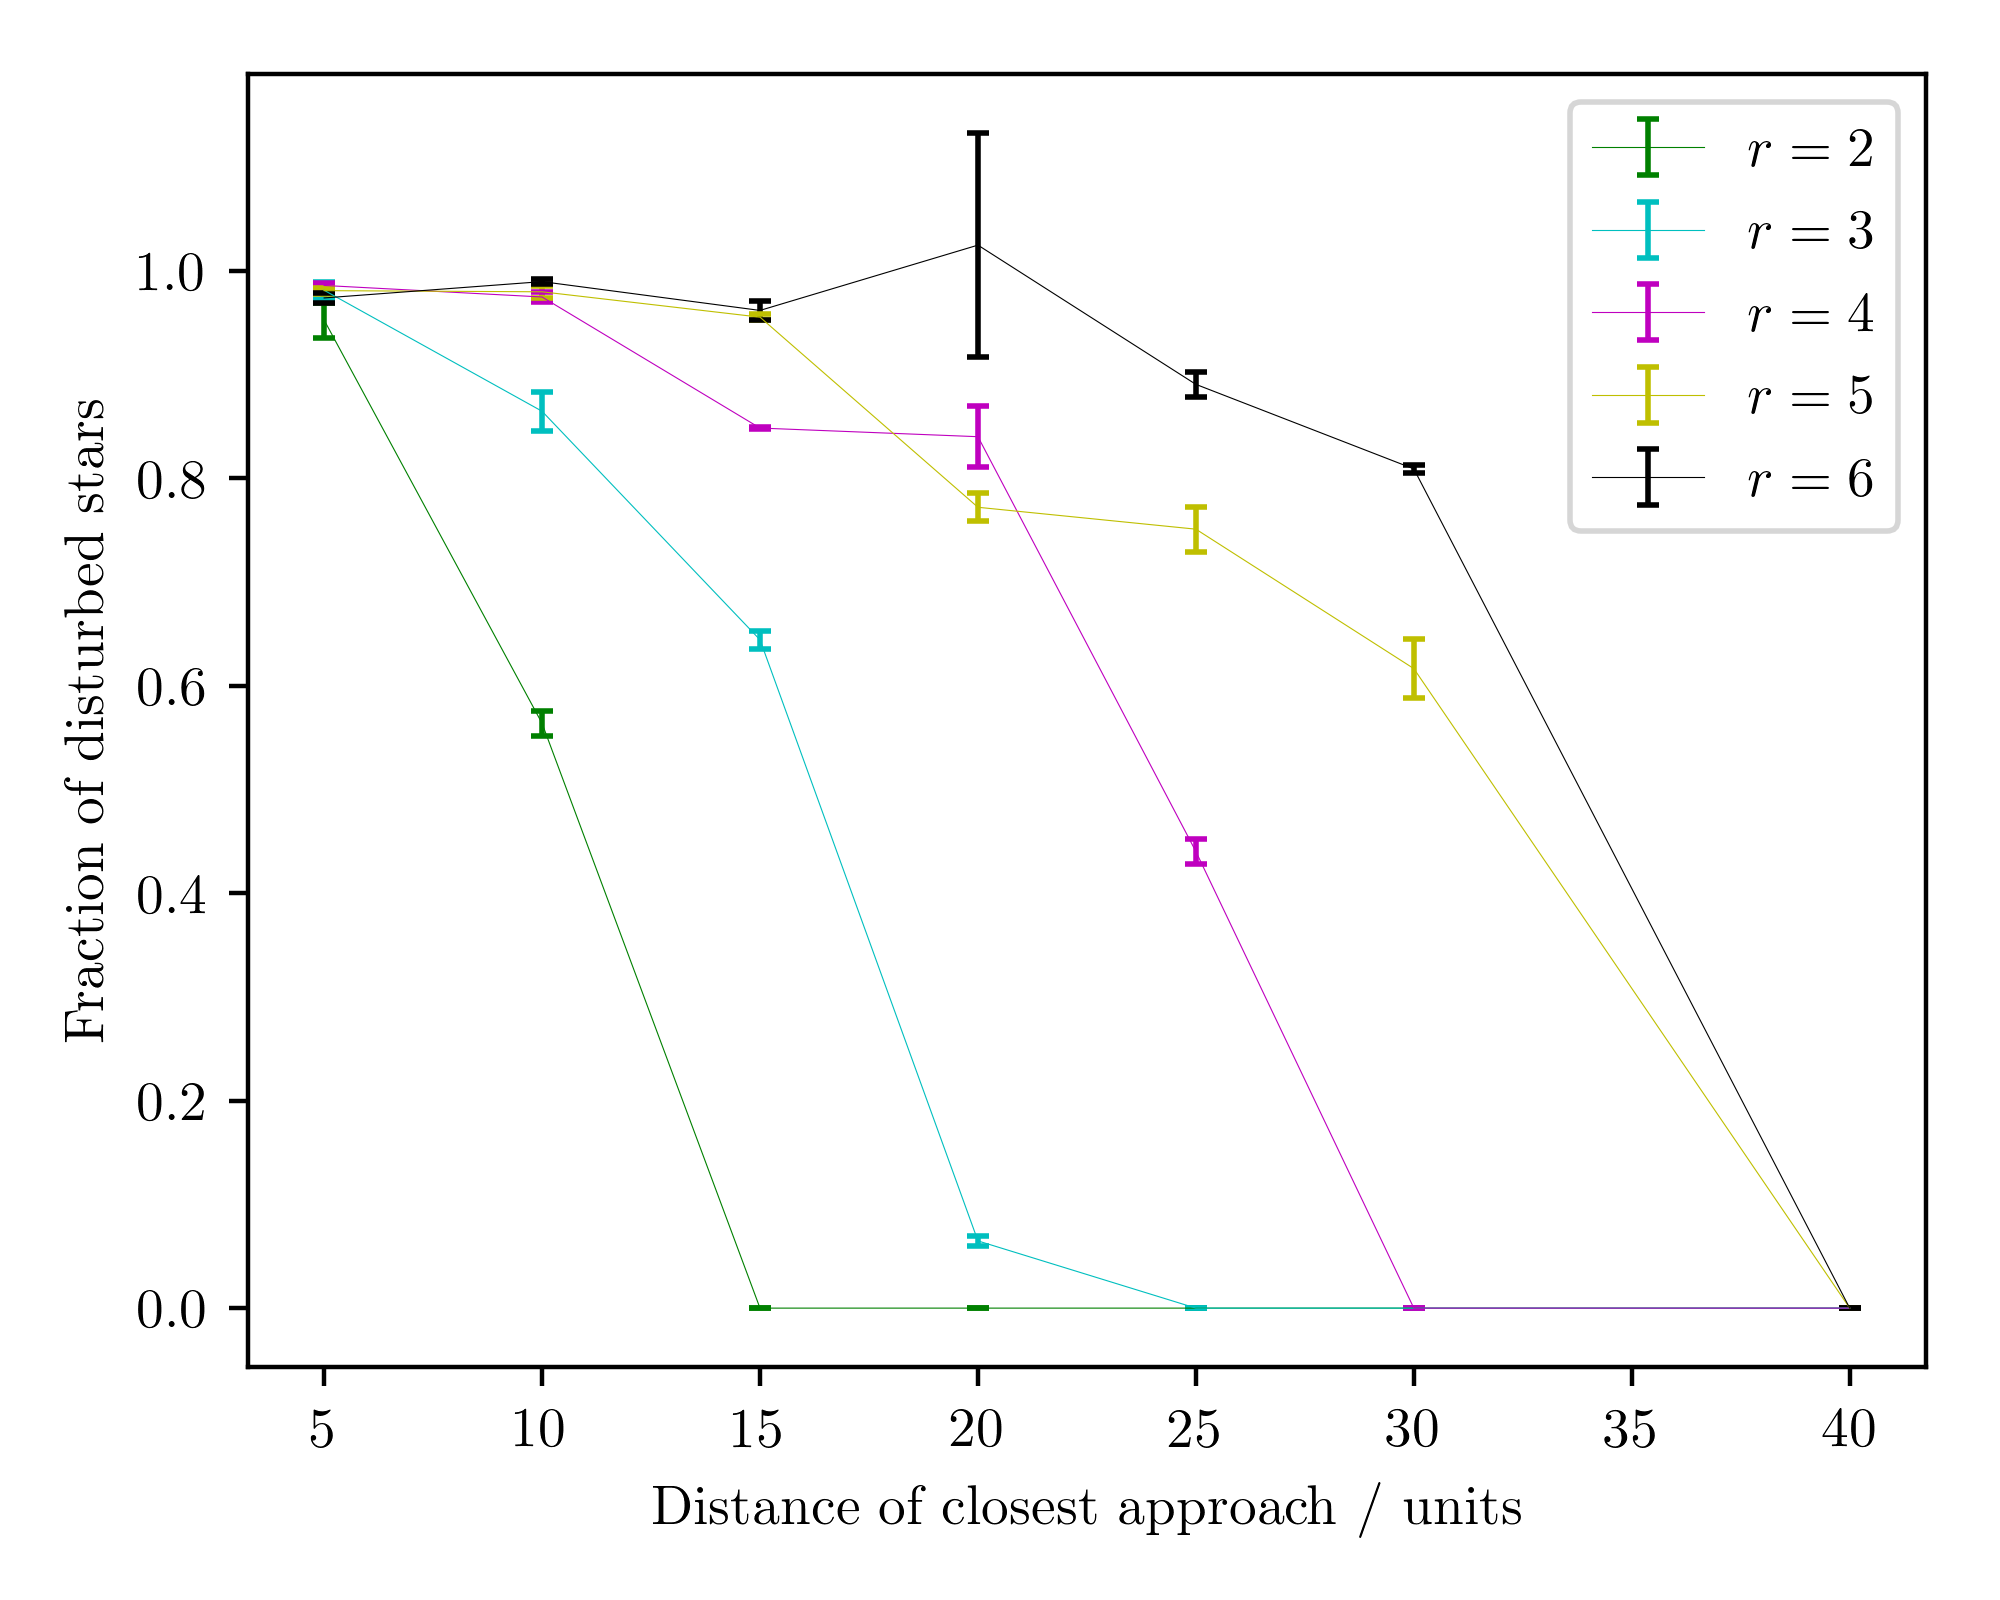
\includegraphics[width=\linewidth]{images/varying_rmin.png}
            \caption{Plots of the fraction of stars disturbed from their initial orbit against the mass of the perturbing galaxy (top plot) and the distance of the closest approach (bottom plot) for each initial orbiting radius.}
            \label{figure:varying}
        \end{figure}

        
        The effects of varying the mass of the perturbing galaxy and varying the distance of closest approach between the two galaxies are shown in Figure \ref{figure:varying} respectively. Both figures show the fraction of stars disturbed from their initial orbits, where 'disturbed' is defined by when the distance between the star and the central galaxy deviates by more than 0.5 units away from its initial orbiting radius. Here, three runs of the simulation were performed for each point, and the errorbars shown are the standard error of the means. 

        It is clear from Figure \ref{figure:varying} that the heavier the mass of the perturbing galaxy the more disruptive it is to the orbiting stars of the central galaxy, and the closer the distance of closest approach the more disruptive the perturbing galaxy is. However, it is difficult to determine the exact relationship of the fraction of disturbed stars against either the mass of the perturbing galaxy or the distance of closest approach. Further experiments would be required to better understand and determine this dependence.
    
    \subsection{Potential Sources of Errors}
        
        The largest source of potential error in this simulation is the use of a finite timestep. It is impossible to achieve an infinitesimally small timestep due to the restrictions of a classical computer, however a sufficiently small finite timestep would create a good and accurate simulation. A timestep that is too large can lead to an inaccurate simulation, and can potentially lead to a divergence of the positions and/or velocities of the simulated particles. The choice of a timestep of \texttt{dt = 0.1} in this simulation was due to the need of balancing the efficiency of the program against the accuracy of the simulation. Given that the timestep method is $\mathcal{O}(N^2)$, decreasing the timestep by a factor of 10 would result in a runtime 100 times longer, which is not ideal!

        Another factor that could lead to large errors occurs when the test particles get very close to the 'core' of the galaxies, where $r$ becomes very small. Given that the acceleration is $\ddot{x} = GM(x - X) / r^3$, this means the acceleration would become very large at small $r$, thus causing the position of the test particles to diverge and 'explode'. This issue can most definitely be mitigated by introducing a finite radius impenetrable to the test particles around the massive galaxies. However, this issue is not a huge factor in the formation of tidal tails in this simulation, thus it was ignored.

        A final, albeit minor, factor for the error of this simulation is the assumption that the test particles were collisionless. Collisions between stars can change the trajectories of the stars and potentially result in a different outcome to the simulation. However, the scale of a galaxy is much bigger than that of a star, and such effects are often negligible in these scenarios. Thus, the assumption of collisionless test particles is a sound assumption in this simulation. 

\section{Conclusion}

        Using the simple timestep method, this simulation was able to successfully simulate close encounters between two galaxies. This simulation was able to emulate part of the results of the simulations performed by Toomre and Toomre in 1972, where prograde encounters were found to be significantly more disruptive than retrograde encounters. The strong tidal effects in retrograde encounters were likely to be the cause of the formation of tidal tails.

        In addition, experiments with this simulation found that the heavier the mass of the perturbing galaxy and the smaller the distance of closest approach is, the more disruptive the perturbing galaxy becomes, displacing a larger proportion of stars from their initial orbits.
    

\onecolumn
\section{Appendix}

{\large \texttt{simulation.py}}
\begin{lstlisting}[language=Python, breaklines=true]
    import matplotlib.pyplot as plt
    import numpy as np
    
    G = 1

    class Body:
        def __init__(self, position, velocity, mass=1, G=G):
            self.mass = mass
            self.G = G
            self.x = position[0]
            self.y = position[1]
            self.v_x = velocity[0]
            self.v_y = velocity[1]
            self.f_x = 0
            self.f_y = 0

        def set_gforce(self, bodies):
            self.f_x = 0
            self.f_y = 0

            for body in bodies:
                d_x = body.x - self.x
                d_y = body.y - self.y
                distance = np.sqrt(d_x**2 + d_y**2)
                force_mag = self.G * body.mass * self.mass / distance**2
                self.f_x += force_mag * d_x / distance
                self.f_y += force_mag * d_y / distance
            
            return self

        def update_speed_position(self, dt):
            self.v_x += dt * self.f_x / self.mass
            self.v_y += dt * self.f_y / self.mass
            self.x += dt * self.v_x
            self.y += dt * self.v_y

            return self


    # initialising the central galaxy
    central_body = Body([0, 0], [0, 0], mass=1)

    # initialising the perturbing galaxy
    # parabolic orbit: y^2 = 4 * r_min^2 - 4 * r_min * x
    r_min = 20
    moving_mass = 1
    moving_x = -50
    moving_y = -2 * np.sqrt(r_min**2 - r_min * moving_x)
    dy_dx = r_min / np.sqrt(r_min**2 - r_min * moving_x)
    moving_v_mag = np.sqrt(2 * G * central_body.mass / np.sqrt(moving_x**2 + moving_y**2))
    moving_v_y = dy_dx * moving_v_mag / np.sqrt(1 + dy_dx**2)
    moving_v_x = moving_v_y / dy_dx
    moving_body = Body([moving_x, moving_y], [moving_v_x, moving_v_y], mass=1)

    # initialising the test particles
    radii_and_units = [
        (2, 120),
        (3, 180),
        (4, 240), 
        (5, 300),
        (6, 360)
    ]
    all_particles = []

    for (radius, num_of_units) in radii_and_units:
        thetas = np.random.rand(num_of_units) * 2 * np.pi
        v_mag = np.sqrt(G * central_body.mass / radius)

        init_x = lambda t : radius * np.cos(t)
        init_y = lambda t : radius * np.sin(t)
        init_v_x = lambda t : -v_mag * np.sin(t)
        init_v_y = lambda t : v_mag * np.cos(t)

        particles = [Body(
            [init_x(theta), init_y(theta)],
            [init_v_x(theta), init_v_y(theta)], 
            mass = 0.01 
        ) for theta in thetas]

        all_particles.append(particles)

    all_particles = [part for radius_particles in all_particles for part in radius_particles]


    dt = 0.1
    t = 0

    with open(f"ac_positions.csv", "w+") as file:

        header = "time,central_x,central_y,moving_x,moving_y"
        for radius, num_of_units in radii_and_units:
            header_str = ",".join([f"particle_{radius}_{i}_x,particle_{radius}_{i}_y" for i in range(num_of_units)])
            header += "," + header_str
        file.write(header + "\n")

        count = 0
        while (t < 700):
            row = str(t) + ","
            
            # update the force, position and velocity of the central galaxy
            central_body.set_gforce([moving_body])
            central_body.update_speed_position(dt)
            row += str(central_body.x) + "," + str(central_body.y)
            
            # update the force, position and velocity of the perturbing galaxy
            moving_body.set_gforce([central_body])
            moving_body.update_speed_position(dt)
            row += "," + str(moving_body.x) + "," + str(moving_body.y)

            # update the force, position and velocity of all the test particles
            all_particles = [part.set_gforce([central_body, moving_body]) for part in all_particles]
            all_particles = [part.update_speed_position(dt) for part in all_particles]
            particle_positions = [str(part.x) + "," + str(part.y) for part in all_particles]
            row += "," + ",".join(particle_positions)

            file.write(row + "\n")

            t += dt
            if count % 500 == 0:
                print(t)

            count += 1
    
\end{lstlisting}

\newpage
{\large \texttt{animation.py}}
\begin{lstlisting}[language=Python, breaklines=true]
    import numpy as np
    import pandas as pd
    import matplotlib.pyplot as plt
    import time

    radii_units_colors = [
        (2, 120, 'g'),
        (3, 180, 'c'),
        (4, 240, 'm'), 
        (5, 300, 'y'),
        (6, 360, 'k')
    ]


    print("Reading file...")
    positions = pd.read_csv(f"ac_positions.csv", delimiter=",")
    print("File read.")

    snapshot_rows = np.linspace(0, len(positions)- 1, 100, dtype=int)
    snapshot_positions = positions.iloc[snapshot_rows,:]

    for idx, row in snapshot_positions.iterrows():
        time = row[0]
        central_x = row[1]
        central_y = row[2]
        moving_x = row[3]
        moving_y = row[4]
        test_particles_positions = row[5:]
        all_test_particles_x = [coord for idx, coord in enumerate(test_particles_positions) if idx % 2 == 0]
        all_test_particles_y = [coord for idx, coord in enumerate(test_particles_positions) if idx % 2 == 1]

        test_particles_xs = []
        test_particles_ys = []
        index = 0
        for (radius, num, color) in radii_units_colors:
            test_particles_xs.append(all_test_particles_x[index:index + num])
            test_particles_ys.append(all_test_particles_y[index:index + num])
            index += num

        plt.clf()
        plt.scatter(central_x, central_y, color='b')
        plt.scatter(moving_x, moving_y, color='r')
        for idx, (radius, num, color) in enumerate(radii_units_colors):
            plt.scatter(test_particles_xs[idx], test_particles_ys[idx], s=1, color=color, label=rf"$r = {radius}$")
            
        plt.xlim([-100, 100])
        plt.ylim([-100, 100])
        plt.pause(0.01)

\end{lstlisting}
\vfill




\bibliography{report}{}
\bibliographystyle{unsrt}

\end{document}
